% Copyright (C) 2010,2011,2012,2013,2014,2015,2016 The ESPResSo project
% Copyright (C) 2002,2003,2004,2005,2006,2007,2008,2009,2010 
%   Max-Planck-Institute for Polymer Research, Theory Group
%  
% This file is part of ESPResSo.
%   
% ESPResSo is free software: you can redistribute it and/or modify it
% under the terms of the GNU General Public License as published by the
% Free Software Foundation, either version 3 of the License, or (at your
% option) any later version.
%  
% ESPResSo is distributed in the hope that it will be useful, but
% WITHOUT ANY WARRANTY; without even the implied warranty of
% MERCHANTABILITY or FITNESS FOR A PARTICULAR PURPOSE.  See the GNU
% General Public License for more details.
%  
% You should have received a copy of the GNU General Public License
% along with this program.  If not, see <http://www.gnu.org/licenses/>.
%
%%%%%%%%%%%%%%%%%%%%%%%%%%%%%%%%%%%%%%%%%%%%%%%%%%%%%%%%%%%%%%%%% 
% From the brainstorming:
%
% Preknowledge:
% 
% Basic MD(simple integrator,langevin thermostat, ---basic tcl
% basic potentials, basis tutorial 1
% 
% Basis Tutorial: written in Latex
% 
% <<every line of script code should be explained>>
% 
% 1) tcl basic setting up a system
% MD, soft sphere and Lennard-Jones Fluid (argon system), 
% Units
% 
% online visualization (pdb output)
% rdf, pressure,energy,
% 
% online analysis function
% savin, readin writeout, offline analysis, statistics
% 
% Structure:
% Part1:
% 1) Prerequisits (what you should know beforehand: basic tcl knowledge,
% Here you can find more info: Allen, Tildesley: Frenkel smit,
% Rappaport, tcl tutorial,
% 
% 2) Physics of the systems (argon, soft sphere system)
% 
% 3) Algorithms (verlocity verlet, Langevin, Potentials, LJ)
% 3b) about units
% 
% Part2 
% 1) simulation script in all detail, line by line
% Initialize
% Visualize
% Simulate (with online analysis, saves for later off-line analysis,
% (Savelize (save our lives ))
% 
% 2) a new script for later
% analysis, and other helper ideas
% 
% Things to remember and take care of:
% Use the same names for variables
% 
% ====================================================================
% General Tutorial: (the next tutorials: pe_solution, cell model of one
% charged colloid, LB, ferrofluid)
% 
\documentclass[
paper=a4,                       % paper size
fontsize=11pt,                  % font size
twoside,                        % two sided
footsepline,                    % add a line to separate the footer
headsepline,                    % add a line to separate the header
headinclude=false,              % header does not belong to the text
footinclude=false,              % footer does not belong to the text
pagesize,                       % set the pagesize in a DVI document
]{scrartcl}

% Copyright (C) 2010,2011,2012 The ESPResSo project
% Copyright (C) 2002,2003,2004,2005,2006,2007,2008,2009,2010
%  Max-Planck-Institute for Polymer Research, Theory Group
%  
% This file is part of ESPResSo.
%   
% ESPResSo is free software: you can redistribute it and/or modify it
% under the terms of the GNU General Public License as published by the
% Free Software Foundation, either version 3 of the License, or (at your
% option) any later version.
%  
% ESPResSo is distributed in the hope that it will be useful, but
% WITHOUT ANY WARRANTY; without even the implied warranty of
% MERCHANTABILITY or FITNESS FOR A PARTICULAR PURPOSE.  See the GNU
% General Public License for more details.
%  
% You should have received a copy of the GNU General Public License
% along with this program.  If not, see <http://www.gnu.org/licenses/>.
%
\usepackage[draft]{varioref}    % defines \vref
\usepackage{hyperref}           % automatically creates links when
                                % using pdflatex, defines \url
\usepackage{ifpdf}              % defines \ifpdf
\usepackage{graphicx}           % handles graphics
\usepackage{color}              % use colors

\usepackage{amsmath}

\usepackage{verbatim}           % required for \verbatim and \endverbatim
\usepackage{fancyvrb}
\usepackage{calc}               % compute length
\usepackage{ifthen}             % provide ifthen
\usepackage{xspace}
\usepackage{units}
\usepackage[numbers]{natbib}

% For building the distribution docs, disable todo boxes.
%\usepackage[disable]{todonotes}
\usepackage{todonotes}

\newcommand{\es}{\mbox{\textsf{ESPResSo}}\xspace}
\newcommand{\ie}{\textit{i.e.}\xspace}
\newcommand{\eg}{\textit{e.g.}\xspace}
\newcommand{\etal}{\textit{et al.}\xspace}

\newcommand{\codebox}[1]%
{\texttt{#1}}

\DefineVerbatimEnvironment{code}{Verbatim}%
{commandchars=\\\{\}}
\makeatletter
\newenvironment{tclcode}
{%
  \addtolength{\linewidth}{-2em}% set the line length
  \@minipagetrue%%%DPC%%%
  \@tempswatrue%%%DPC%%%
  \hsize=\linewidth%
  \setbox0=\vbox\bgroup\verbatim
}{\endverbatim
  \unskip\setbox0=\lastbox%%%DPC%%%
  \egroup
  \par%
  \noindent\hspace{1em}%
  \codebox{\box0}%
  \par\noindent%
}
\makeatother

% \newcommand{\todo}[1]{
%   \marginpar{%
%     \setlength{\fboxrule}{1pt}
%     \fcolorbox{red}{yellow}{%
%       \parbox{\marginparwidth-2\fboxrule-2\fboxsep}{%
%         \bf\raggedright\scriptsize #1%
%       }%
%     }%
%   }%
% }

\makeatletter
\renewcommand{\minisec}[1]{\@afterindentfalse \vskip 1.5ex
  {\parindent \z@
    \raggedsection\normalfont\sffamily\itshape\nobreak#1\par\nobreak}%
  \@afterheading}
\makeatother

\newcommand{\esptitlehead}{
  \titlehead{
    \begin{center}
      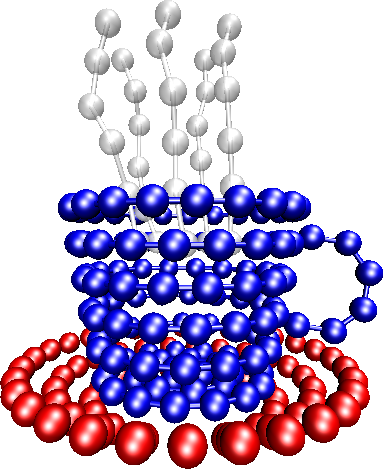
\includegraphics[width=5cm]{logo/transparentbg}
    \end{center}
  }
}

% \newcommand{\es}{ESPResSo}
%% Grafikpakete
\usepackage{graphicx}%
\usepackage{siunitx}% To typeset numbers and units

\usepackage{verbatim}

% How to diplay ESPResSo commands in flowing text. Larger code segments
% should be put inside boxes.
\newcommand{\EScmd}[1]{\texttt{\textbf{#1}}}

% The code block
%\newcommand{\EScode}[1]{ \parbox{0.95\textwidth}{\texttt{#1}}}
\usepackage{listings} 
\lstset{numbers=left, numberstyle=\tiny, numbersep=5pt, showspaces=false, showstringspaces=false,postbreak=\space, breakindent=5pt, breaklines}
\lstset{language=python, keywordstyle=\color{blue}\bfseries ,emphstyle=\color{green}, commentstyle=\color{red}\itshape }
\lstset{keywordsprefix=setmd}
\lstset{keywords=[6]{thermostat,part,inter,integrate,rescale_velocities,code_info,save_sim,writepdb,analyze,uwerr}}

\newtheorem{task}{Task}

\begin{document}


\title{Tutorial: Raspberry Electrophoresis%
\ifdefined\esversion%
\thanks{For \es \esversion}%
\fi%
}
\subtitle{\es Basics}
\author{O.A. Hickey \and S. Raafatnia}
\maketitle


\section{Tutorial Outline}

Welcome to the raspberry electrophoresis \es{} tutorial! This tutorial assumes some basic knowledge of \es{}.
The first step is compiling \es{} with the appropriate flags, as listed in Sec.~\ref{sec:compiler_flags}.
The tutorial starts by discussing how to build a colloid out of a series of MD beads. These particles typically
ressemble a raspberry as can be seen in Fig.~\ref{fig:rasp_snapshot}. After covering the construction of a raspberry colloid, we then
briefly discuss the inclusion of hydrodynamic interactions via a lattice-Boltzmann fluid. Finally we will cover
including ions via the restrictive primitive model (hard sphere ions) and the addition of an electric field
to measure the electrokinetic properties. A working Python script is also provided in the file scripts/simulate\_raspberry\_electrophoresis.py. Running
this script will run a raspberry electrophoresis simulation and write the time and position of the colloid out to a file named posVsTime.dat in the same directory.
A sample set of data is included in the file posVsTime\_sample.dat.

\begin{figure}[]
	\centering
	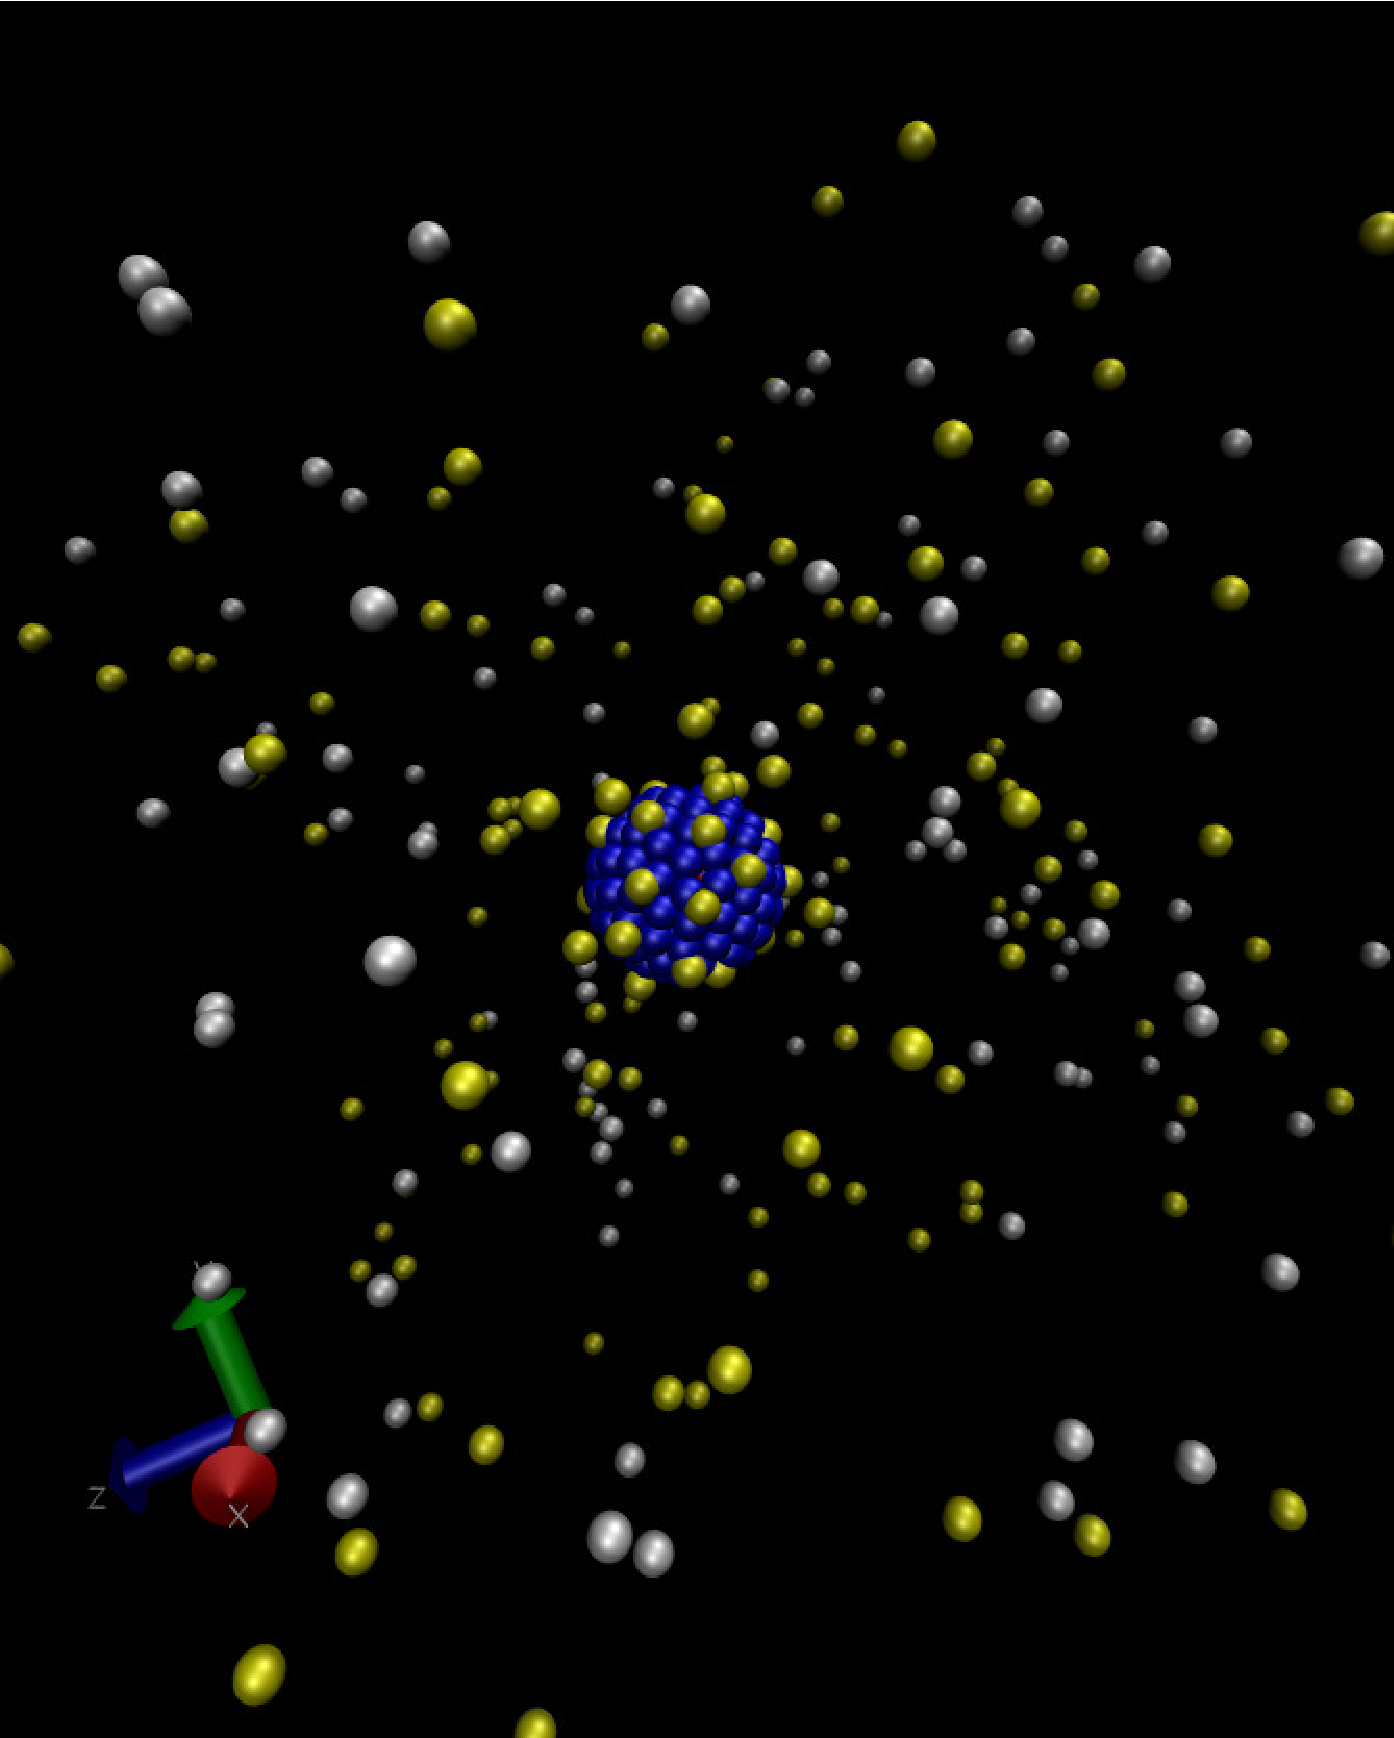
\includegraphics[width=\linewidth]{figures/raspberry_snapshot}
	\caption{A snapshot of the simulation consisting of positive salt ions (yellow spheres), negative salt ions (grey spheres) and surface beads (blue spheres). There is also a central bead in the middle of the colloid bearing a large negative  charge.}
	\label{fig:rasp_snapshot}
\end{figure} 

\section{Compiling ESPResSo for this Tutorial}\label{sec:compiler_flags}
The first thing with any \es{} project is to compile \es{} with all of the necessary features.
The following myconfig.hpp example contains all of the flags needed for running the accompanying Python script.
Please compile \es{} using this myconfig.hpp before starting this tutorial.
{\small\vspace{0,2cm}
\begin{lstlisting}[numbers=none]
/* Necessary Flags for the ESPResSo Raspberry Tutorial */

#define ELECTROSTATICS
#define ROTATION
#define ROTATIONAL_INERTIA
#define EXTERNAL_FORCES
#define MASS
#define BOND_VIRTUAL
#define VIRTUAL_SITES_RELATIVE
#define LB_GPU
#define LENNARD_JONES
\end{lstlisting}\vspace{0,2cm}
}
\section{Global MD Variables}\label{sec:espresso}

  The first thing in any \es{} simulation is to set a few global simulation parameters:

{\small\vspace{0,2cm}
\begin{lstlisting}
system = espressomd.System()
system.box_l = [box_l, box_l, box_l]
\end{lstlisting}\vspace{0,2cm}
}

The parameter $box\_l$ sets the size of the simulation box. In general, one should check for finite
size effects which can be surprisingly large in simulations using hydrodynamic interactions. They
also generally scale as $box\_l^{-1}$ or $box\_l^{-3}$ depending on the transport mechanism
which sometimes allows for the infinite box limit to be extrapolated to, instead of using an
excessively large simulation box. As a rule of thumb, the box size should be five times greater than the characteristic
length scale of the object. 
{\small\vspace{0,2cm}
\begin{lstlisting}[numbers=none]
system.time_step = time_step
\end{lstlisting}\vspace{0,2cm}
}
The parameter $time\_step$, which represents the time step used in the Verlet
integration, should generally be chosen to be as large as possible, while still producing the same numerical
values of the physical properties being measured. In typical coarse-grained simulations as
covered in this tutorial, this value turns out to be $time\_step=0.01$.
{\small\vspace{0,2cm}
\begin{lstlisting}[numbers=none]
system.skin = skin
\end{lstlisting}\vspace{0,2cm}
}
 The skin is used for constructing
the Verlet lists and is purely an optimization parameter. Whatever value provides the fastest
integration speed should be used. For the type of simulations covered in this tutorial, this value turns out
to be $skin \approx 0.3$.
{\small\vspace{0,2cm}
\begin{lstlisting}[numbers=none]
system.periodicity = [1, 1, 1]
\end{lstlisting}\vspace{0,2cm}
}
The $periodicity$ parameter indicates that the system is periodic in all three
dimensions. Note that the lattice-Boltzmann algorithm requires periodicity in all three directions (although
this can be modified using boundaries, a topic not covered in this tutorial). 

\section{Setting up the Raspberry}

Setting up the raspberry is a non-trivial task. The main problem lies in creating a relatively
uniform distribution of beads on the surface of the colloid. In general one should take about 1 bead per grid
point on the surface to ensure that there are no holes in the surface. The behavior of the colloid can be further improved by placing
beads inside the colloid, though this is not done in this example script. In our example
we first define a center of the colloid, a harmonic interaction causing the surface beads to be attracted
to the center, and a Lennard-Jones interaction preventing the beads from entering the colloid. There is also a Lennard-Jones
potential between the surface beads to get them to distribute evenly on the surface. 

The beads are initialized at random positions on the surface of the colloid. The beads are then allowed to relax using
an integration loop where the forces between the beads are capped. The best way to ensure a relatively uniform distribution
of the beads on the surface is to simply take a look at a VMD snapshot of the system after this integration. As can
be seen in Fig.~\ref{fig:rasp_snapshot}.

In order to make the colloid perfectly round we now adjust the beads positions to be exactly $radius\_col$ away
from the central bead.
Now that the beads are arranged in the shape of a raspberry, the surface beads are virtualized. The central
bead is also given an appropriate mass and moment of inertia tensor (note that the off-diagonal elements
are zero in \es{}'s implementation). Lastly the central bead is given the total electrostatic charge on the colloid. In principle
one could also assign the charge to the surface beads, which might be more realistic, but would require more computational
effort for calculating the electrostatic interactions.

\section{Inserting Counterions and Salt Ions}

Next we insert enough ions at random positions (outside the radius of the colloid) with opposite charge to the colloid such that the system is electro-neutral. In addition ions
of both signs are added to represent the salt in the solution. Between all of the ions is the WCA potential, a purely repulsive
version of the Lennard-Jones potential which approximates hard spheres or radius $\sigma$. The ions also have a WCA potential
with the central bead of the colloid with an offset of around $radius\_col-\sigma +a_\mathrm{grid}/2$. This make
the colloid appear as a hard sphere of radius roughly $radius\_col+a_\mathrm{grid}/2$ to the ions, which is roughly equal to the
hydrodynamic radius of the colloid. After inserting the ions, again a short integration is performed with a force cap to
prevent strong overlaps between the ions.

\section{Electrostatics}
Electrostatics are simulated using the Particle-Particle Particle-Mesh (P3M) algorithm. In \es{} this can be added to the simulation rather trivially:
{\small\vspace{0,2cm}
\begin{lstlisting}[numbers=none]
p3m = electrostatics.P3M(bjerrum_length=bjerrum, accuracy=0.001)
system.actors.add(p3m)
\end{lstlisting}
}
Generally a Bjerrum length of $2$ is appropriate when using WCA interactions with $\sigma=1$ since a typical ion has a radius of $\SI{0.35}{nm}$, while the Bjerrum
length in water is around $\SI{0.7}{nm}$.

The external electric field is simulated by simply adding a constant force equal to the simulated field times the particle charge. Generally the electric field is set to $0.1$ in MD units
which is the maximum field before the response becomes nonlinear. Smaller fields are also possible, but the required simulation time is considerably larger. Sometimes, Green-Kubo methods
are also used, but these are generally only feasible in cases where there is either no salt or a very low salt concentration.

\section{Lattice-Boltzmann}
The lattice-Boltzmann (LB) fluid can be easily create in \es{} using the $LBFluid$ command.
Before creating the LB fluid it is a good idea to set all of the particle velocities to zero via the $kill\_particle\_motion()$ command.
This is necessary to set the total momentum of the system to zero. Failing to do so will lead to an unphysical drift of the system, which
will change the values of the measured velocities.

The important parameters for the LB fluid are the density, the viscosity, the time step and the friction. The time step should generally be comparable to the MD time step. While
large time steps are possible, a time step of $0.01$ turns out to provide more reasonable values for the root mean squared particle velocities. Both density and viscosity
should be around $1$, while the friction should be set around $20.$ The grid spacing should be comparable to the ions' size.
{\small\vspace{0,2cm}
\begin{lstlisting}[numbers=none]
system.galilei.kill_particle_motion()
lb = espressomd.lb.LBFluid_GPU(dens=1., visc=3., agrid=1., tau=time_step, fric=20)
system.actors.add(lb)
\end{lstlisting}
}

A logical way of picking a specific set of parameters is to choose them such that the hydrodynamic radius of an ion roughly matches its physical radius determined by the
WCA potential ($R=0.5\sigma$). Using the following equation:
\begin{equation}
\frac{1}{\Gamma}=\frac{1}{6\pi \eta R_{\mathrm{H0}}}=\frac{1}{\Gamma_0} 
+\frac{1}{g\eta a} 
 \label{effectiveGammaEq}
\end{equation}
one can see that the set of parameters grid spacing $a=1\sigma$, fluid density $\rho=1$, a 
kinematic viscosity of $\gamma=3 $ and a friction of $\Gamma_0=50$ leads to a hydrodynamic radius
of approximately $0.5\sigma$.

The last step is to first turn off all other thermostats, followed by turning on the LB thermostat. The temperature is typically set to 1, which is equivalent to setting
$k_\mathrm{B}T=1$ in molecular dynamics units.

{\small\vspace{0,2cm}
\begin{lstlisting}[numbers=none]
system.thermostat.turn_off()
system.thermostat.set_lb(kT=1.)
\end{lstlisting}
}

\section{Simulating Electrophoresis}
Now the main simulation can begin! The only important thing is to make sure the system has enough time to equilibrate. There are two separate equilibration times: 1) The time for the ion distribution to stabilize, and 2) The time
needed for the fluid flow profile to equilibrate. In general, the ion distribution equilibrates fast, so the needed warmup time is largely determined by the fluid relaxation time, which can be calculated via $\tau_\mathrm{relax} = box\_length^2/\nu$. This means for a box of size 48 with a kinematic viscosity of 3 as in our example script, the relaxation time is $\tau_\mathrm{relax} = 48^2/3 = 768 \tau_\mathrm{MD}$, or 76800 integration steps. In general it is a good idea to run for many relaxation times before starting to use the simulation results for averaging observables. To be on the safe side $10^6$ integration steps is a reasonable equilibration time. Please feel free to modify the provided script and try and get some interesting results!
\end{document}

